\documentclass{article}

\usepackage{graphicx}
\usepackage{subfig}
\usepackage{amsmath}

\title{Two-dimensional Helium Plume}

\date{}

\begin{document}

\maketitle

\section{Introduction}
This case provides a description for a two-dimensional helium plume 
configuration. A mixture fraction is activated that drives mixing and 
buoyant effects. Although the full physics description can only be 
represented by a three-dimensional domain, nevertheless, the case 
captures common instabilities found in buoyant plumes such as 
Rayleigh/Taylor and Kelvin/Helmholtz phenomena. The baroclinic 
torque noted in the flow drives the large-scale vortical motion. For 
more details on the physics of buoyant plumes and fires, 
see Tieszen's seminal work in fire research~\cite{tieszenReview} and 
a recent fire validation study of Domino \textit{et al.}~\cite{dominoPoF2021}.
Finally, although the plume enters into the domain as a laminar inflow 
condition, there exists laminar-to-turbulent transition inspired by 
the buoyant vertical acceleration. Again, a simplification of this 
simulation is the under-resolved nature along with an absent turbulence model.

\section{Domain}
The two-dimensional geometry for this tutorial is captured in 
Figure~\ref{fig:geom}. Here, pure helium enters a 1 $m$ inflow boundary
that is surrounded by a bottom wall plane that is six meters in width
and five meters in height. The left and right boundaries are open boundaries
where entrainment is expected, while the top is also an open boundary
specification where flow leaves the domain. Due to complex vortical flow,
the top open boundary experiences periodic entrainment as complex structures
exit the domain.

\begin{figure}[!htbp]
  \centering
  {
   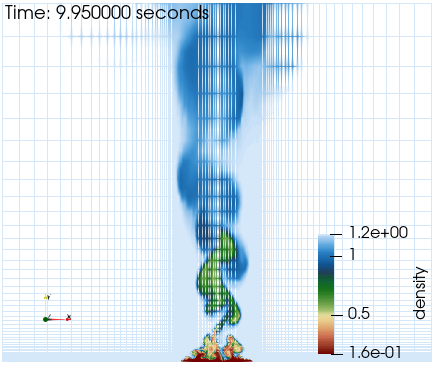
\includegraphics[height=2.0in]{images/2d_quad9_helium_geom.png}
  }
  \caption{Two-dimensional helium plume configuration. The wire diagram 
outlines the quadratic Quad9 mesh and density shadings.}
  \label{fig:geom}
\end{figure}

\section{Theory}
The variable-density low-Mach equation set is defined by the continuity 
and momentum equation,

\begin{align}
  \frac {\partial \rho }{\partial t} + \frac{ \partial \rho u_j}{\partial x_j} = 0.
\label{eq:contEq}
\end{align} 

\begin{align}
  \frac {\partial \rho u_i }{\partial t} + \frac{ \partial \rho u_j u_i}{\partial x_j} 
-\frac{\partial \sigma_{ij}}{\partial x_j} = \left( \rho - \rho^o \right) g_i.
\label{eq:momEq}
\end{align}
%
In the above equation, $\rho$ is the fluid density and $u_j$ is the 
fluid velocity. The buoyancy source term is given by the difference 
between the local density and reference density, $\rho^o$, scaled 
by gravity, $g_i$.

The stress tensor is provided by
\begin{align}
\sigma_{ij}  = 2 \mu S^*_{ij} - P \delta_{ij},
\end{align}
%
where the traceless rate-of-strain tensor is defined as
\begin{align}
S^*_{ij}  = S_{ij} - \frac{1}{3} \delta_{ij} S_{kk} \nonumber
		     = S_{ij} - \frac{1}{3} \frac{\partial  u_k }{\partial x_k}\delta_{ij}.
\end{align}
In a low-Mach flow, the above pressure, $P$, is the perturbation about 
the thermodynamic pressure, $P^{th}$. 

For the buoyant plume configuration of interest, a transport equation 
for mixture fraction is activated and defined as the mass fraction of 
species that originates from the inlet boundary condition,

\begin{align}
  \frac {\partial \rho Z }{\partial t} + \frac{ \partial \rho u_j Z}{\partial x_j} 
+\frac{\partial q_j }{\partial x_j} = 0,
\label{eq:zEq}
\end{align}
where the diffusive flux vector is given by $q_j = -\frac{\mu}{Sc}\frac{\partial Z}{\partial x_j}$.
Here, the Schmidt number is given as a function of density and mass 
diffusivity $D$, as $Sc = \frac{\mu}{\rho D}$. Properties such as viscosity 
are a linear function of mixture fraction, while density uses inverse weighting.

\section{Results}
This simulation is based on the experimental work of O'Hern~\cite{ohern2005} 
where the complex nature of a buoyant plume was studied as a precursor to 
fire simulations~\cite{dominoPoF2021}. In this flow, large-scale vortical 
structure is motivated by the baroclinic torque term (mis-alignment of 
density and pressure gradients) that drives rotation. Rayleigh/Taylor 
instabilities (bubble-spike) are captured that drives small-scale mixing. 

\subsection{Simulation Specification and Results}
The simulation activates a Quad9 topology. Inflow of helium (mixture 
fraction of unity) enters the domain at 0.34 $m/s$ in the y-direction. 
In Figure~\ref{fig:results}, the transient density field is provided
along with time-mean Reynolds-averaged quantities of interest.

\begin{figure}[!htbp]
  \centering
 \subfloat[]
  {
   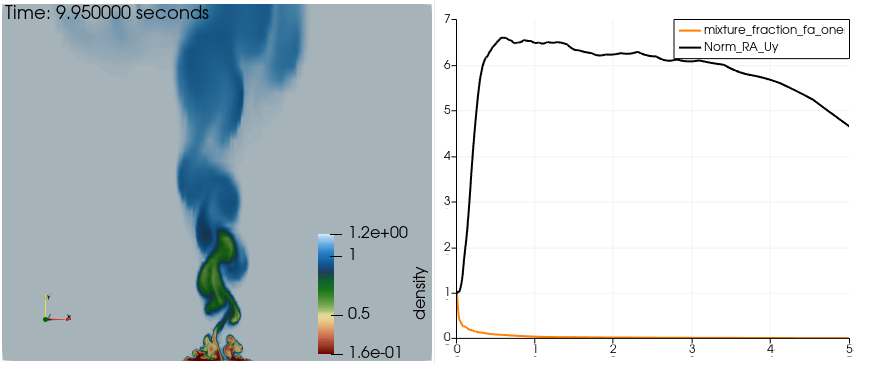
\includegraphics[height=1.5in]{images/2d_quad9_helium_centerline.png}
  }
  \caption{Density shading (left) and centerline plot of Reynolds-averaged 
mixture fraction and normalized axial velocity (right).}
  \label{fig:results}
\end{figure}

\section{Discussion Points}

There are several interesting activities associated with this sample case 
including the following:

\begin{itemize}
	\item Ensure that the underlying model suite is well understood.
	\item Explore the mesh and input file specifications associated 
          with this case.
        \item Please comment on the form of the buoyancy source term and
          how this drives the pressure specification in the input file.
	\item Note the puffing structure and Rayleigh/Taylor instability.
	\item What is a good time-averaging interval to use in this 
          simulation. Note that correlation-based approaches for the 
          temporal puffing frequency is roughly 
          $\frac{1.5}{\sqrt(d_o)}$.
        \item Please comment on the issues with running a two-dimensional 
          configuration for this physics-set. What about the lack of 
          a turbulence model activated in the configuration?
\end{itemize}

\begin{thebibliography}{100}

\bibitem{tieszenReview} Tieszen, S., \emph{On the fluids mechanics of fires}, Annual Review of Fluid Mechanics, Vol. 33, 2001.

\bibitem{dominoPoF2021} Domino, S. P., Hewson, J., Knaus, R., Hansen, M., \emph{Predicting large-scale pool fire dynamics using an unsteady flamelet- and large-eddy simulation-based model suite}, Physics of Fluids, Vol. 33, 2021.

\bibitem{ohern2005} O'Hern, T., Weckman, E., Gerhart, A., Tiezen, S.,  Sheffer, R., \emph{"Experimental study of a turbulent buoyant helium plume}, Journal of Fluid Mechanics, Vol. 544, 2005.

\end{thebibliography}

\end{document}
